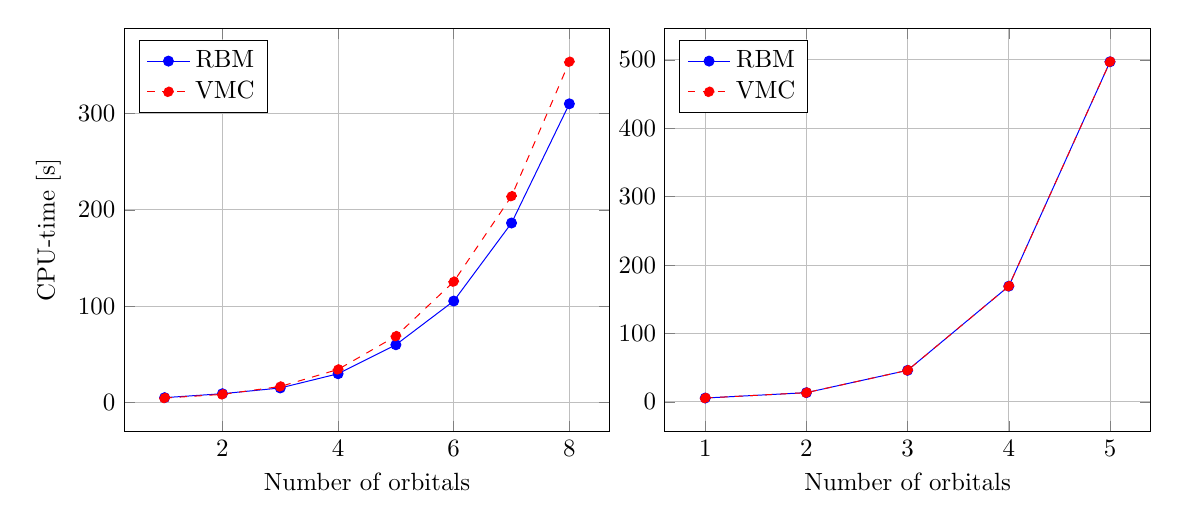
\begin{tikzpicture} [scale=0.9]
	\begin{axis}[name=2D, xlabel=Number of orbitals, ylabel={CPU-time [s]}, grid=major, legend pos=north west] 
	  \addplot[color=blue,mark=oplus*] coordinates { 
	  	 (1,5.141258)
	  	 (2,9.239086)
		 (3,15.17534) 
		 (4,29.92524) 
		 (5,60.01942) 
		 (6,105.3550) 
		 (7,186.3048)
		 (8,309.9558) }; 
	  \addlegendentry{RBM};
	  
	  \addplot[color=red,mark=oplus*, dashed] coordinates { 
	  	(1,4.7485)
	  	(2,8.551862)
	  	(3,16.69836) 
	  	(4,34.40414) 
	  	(5,68.92126) 
	  	(6,125.4514) 
	  	(7,214.0844)
	  	(8,353.5306) }; 
	  \addlegendentry{VMC};
	 \end{axis} 
	 \begin{axis}[name=3D, at=(2D.right of south east), anchor=left of south west, xlabel=Number of orbitals, grid=major, legend pos=north west] 
	 \addplot[color=blue,mark=oplus*] coordinates { 
	 	(1,5.490018)
	 	(2,13.35986)
	 	(3,46.03914) 
	 	(4,169.0882) 
	 	(5,497.2244) }; 
	 \addlegendentry{RBM};
	 
	 \addplot[color=red,mark=oplus*, dashed] coordinates { 
	 	(1,5.490018)
	 	(2,13.35986)
	 	(3,46.03914) 
	 	(4,169.0882) 
	 	(5,497.2244) };
	 \addlegendentry{VMC};
   \end{axis} 
\end{tikzpicture}